\documentclass[12pt]{article}
\usepackage[utf8]{inputenc}
\usepackage{float}
\usepackage{amsmath}
\usepackage[shortlabels]{enumitem}

\usepackage[hmargin=3cm,vmargin=6.0cm]{geometry}
\usepackage{tikz}
%\topmargin=0cm
\topmargin=-2cm
\addtolength{\textheight}{6.5cm}
\addtolength{\textwidth}{2.0cm}
%\setlength{\leftmargin}{-5cm}
\setlength{\oddsidemargin}{0.0cm}
\setlength{\evensidemargin}{0.0cm}
%misc libraries goes here

\begin{document}

\section*{Student Information } 
%Write your full name and id number between the colon and newline
%Put one empty space character after colon and before newline
Full Name : Berk Ulutaş \\
Id Number : 2522084 \\

% Write your answers below the section tags
\section*{Answer 1}
\begin{enumerate}[a)]
    \item False. All real numbers are uncountably infinite, but strings over alphabet $\Sigma = \{0,1,2,\dots,9\}$ namely $\Sigma^* $ countably infinite, and therefore there are uncountably many real numbers that cannot be represented as strings over $\Sigma$.
    \item False. Set of strings over an alphabet $\Sigma^*$ is countably infinite. This means possible representations of languages are countably infinite. Conversely, set of all possible languages over an alphabet $2^{\Sigma^*}$ is uncountably infinite. Therefore we cannot represent uncountable number of things with countable number of representations.
    \item True. $bba \in \mathcal{L}$ we can create this string from $a^*b^*a^*b^*$ with 0-$a$, 2-$b$, 1-$a$, and 0-$b$. 
    \item False. It does not only represent strings that has ab as prefix. $a^+b^+(a \bigcup b)^*$ also creates $aab$. 
    
\end{enumerate}


\section*{Answer 2}
\begin{enumerate}[a)]
    \item
    \begin{itemize}
        \item $K = \{ q_0, q_1, q_2, q_3\}$ 
        \item $\Sigma = \{a,b\}$
        \item $s = q_0$
        \item $F = \{q_0,q_1,q_2\}$
        \item $\delta:$ 
        \begin{tabular}{c|c|c}
            & a & b \\
            \hline
            $q_0$ & $q_1$ & $q_0$ \\
            $q_1$ & $q_1$ & $q_2$ \\
            $q_2$ & $q_3$ & $q_0$ \\
            $q_3$ & $q_3$ & $q_3$ \\
        \end{tabular}
        
    \end{itemize}

\begin{center}
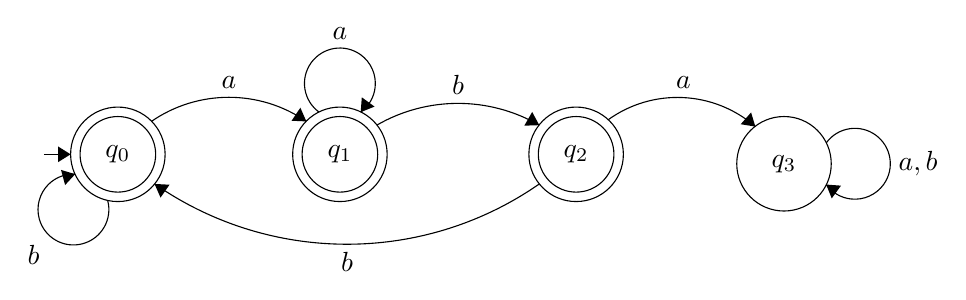
\begin{tikzpicture}[scale=0.2]
\tikzstyle{every node}+=[inner sep=0pt]
\draw [black] (10.6,-26.2) circle (3);
\draw (10.6,-26.2) node {$q_0$};
\draw [black] (10.6,-26.2) circle (2.4);
\draw [black] (24.7,-26.2) circle (3);
\draw (24.7,-26.2) node {$q_1$};
\draw [black] (24.7,-26.2) circle (2.4);
\draw [black] (39.7,-26.2) circle (3);
\draw (39.7,-26.2) node {$q_2$};
\draw [black] (39.7,-26.2) circle (2.4);
\draw [black] (52.9,-26.8) circle (3);
\draw (52.9,-26.8) node {$q_3$};
\draw [black] (12.73,-24.109) arc (124.56296:55.43704:8.672);
\fill [black] (22.57,-24.11) -- (22.19,-23.24) -- (21.63,-24.07);
\draw (17.65,-22.08) node [above] {$a$};
\draw [black] (27.045,-24.346) arc (119.99853:60.00147:10.311);
\fill [black] (37.36,-24.35) -- (36.91,-23.51) -- (36.41,-24.38);
\draw (32.2,-22.46) node [above] {$b$};
\draw [black] (41.724,-24.013) arc (125.81574:48.97913:7.538);
\fill [black] (51.08,-24.44) -- (50.81,-23.54) -- (50.15,-24.29);
\draw (46.52,-22.05) node [above] {$a$};
\draw [black] (55.58,-25.477) arc (144:-144:2.25);
\draw (60.15,-26.8) node [right] {$a,b$};
\fill [black] (55.58,-28.12) -- (55.93,-29) -- (56.52,-28.19);
\draw [black] (37.365,-28.08) arc (-55.1834:-124.8166:21.394);
\fill [black] (12.93,-28.08) -- (13.31,-28.95) -- (13.88,-28.13);
\draw (25.15,-32.41) node [below] {$b$};
\draw [black] (9.95,-29.117) arc (15.17018:-272.82982:2.25);
\draw (5.25,-31.95) node [below] {$b$};
\fill [black] (7.89,-27.46) -- (6.99,-27.19) -- (7.25,-28.15);
\draw [black] (5.9,-26.2) -- (7.6,-26.2);
\fill [black] (7.6,-26.2) -- (6.8,-25.7) -- (6.8,-26.7);
\draw [black] (23.377,-23.52) arc (234:-54:2.25);
\draw (24.7,-18.95) node [above] {$a$};
\fill [black] (26.02,-23.52) -- (26.9,-23.17) -- (26.09,-22.58);
\end{tikzpicture}
\end{center}

    \item \begin{itemize}
        \item  $$(q_0, abbaabab) \vdash_M (q_1, bbaabab) \vdash_M (q_2, baabab) \vdash_M (q_0, aabab) \vdash_M  (q_1, abab) $$
$$\vdash_M (q_1, bab) \vdash_M (q_2, ab) \vdash_M (q_3, b) \vdash_M (q_3, e)$$

        \item No. DFA finishes with state $q_3$ and $q_3$ not in accepted states so it does not accept the input.
    \end{itemize}
    
    
    
\end{enumerate}


\section*{Answer 3}
\begin{enumerate}[a)]
    \item 
        \begin{itemize}
            \item $E(q_0) = \{q_0, q_2\}$
            \item $E(q_1) = \{q_1\}$
            \item $E(q_2) = \{q_2\}$
            \item $E(q_3) = \{q_0,q_2,q_3\}$
            \item $E(q_4)  = \{q_0,q_2,q_3,q_4\}$
        \end{itemize}
    \item 
        \begin{enumerate}[1)]
            \item Define $K'$ as the set consisting of all subsets of K. (It is correct $K'=2^K$)
            \item Define the alphabet $\Sigma'$ as precisely the set $\Sigma$. (It is correct)
            \item Define the set of starting states, $s'$ as set whose only element is s. (It is also correct since question says that It is known that $M$ does not have any empty transitions from its starting state. But to generalize instructions we can say Define the set of starting states, $s'$ as $E(s)$)
            \item Define the set of final states, $F'$ as those elements of $K'$ which consists of only the states $q \in F$. (There is a mistake here. It should be Define the set of final states, $F'$ as those elements of $K'$ which contain at least one state from $F$.)
            \item Define the transition function $\delta$ as taking two inputs: an element $Q$ of $K'$ and an element of $a$ of $\Sigma'$. The function returns the set whose elements are precisely those states $p$ in $K$ for which there exists a $q \in Q$ and $(q,a,p) \in \Delta$. (There is another mistake here. It should be Define the transition function $\delta$ as taking two inputs: an element $Q$ of $K'$ and an element of $a$ of $\Sigma'$. The function returns the set whose elements are precisely those states $E(p)$ where $p$ in $K$ for which there exists a $q \in Q$ and $(q,a,p) \in \Delta$).
        \end{enumerate}

    
\end{enumerate}


\end{document}
